\documentclass[fleqn,10pt,lineno]{wlpeerj}

\usepackage{amsmath}
\usepackage{amssymb}
\usepackage{booktabs}
\usepackage{multirow}
\usepackage{placeins}
\usepackage{float}
\usepackage{flafter}
\usepackage{microtype}
\usepackage{url}
\usepackage[authoryear,round]{natbib}
\usepackage{hyperref}
\usepackage{graphicx}
\usepackage{iftex}

\ifPDFTeX
\else
  \usepackage{fontspec}
  \setmainfont{TeX Gyre Termes}
  \setsansfont{TeX Gyre Heros}
  \setmonofont{Latin Modern Mono}
\fi

\let\cite\citep

\graphicspath{{../}{figures/}{../figures/}}

\title{Matrix-Residual Graph Neural Networks for Graph Classification}

\author[1]{Xuelin Hu}
\author[2]{Xiaoqin Fu}

\affil[1]{School of Railway Communication and Signaling Engineering, Liuzhou Railway Vocational Technical College, Liuzhou 545000, China}
\affil[2]{School of Railway Locomotive and Rolling Stock, Liuzhou Railway Vocational Technical College, Liuzhou 545000, China}

\corrauthor[2]{Xiaoqin Fu}{fuxiaoqin@ltzy.edu.cn}

\begin{abstract}
\textbf{Background.} Residual connections are widely used to stabilize graph neural networks, but residual design is often treated as a one-dimensional depth-wise choice. Multi-branch graph classifiers create a richer design space: residual information can flow along depth, across branches, or through a local two-dimensional branch-by-layer neighborhood.

\textbf{Methods.} We study Matrix-Residual Graph Neural Networks as a controlled residual-topology framework for graph classification. The model family represents hidden states on a branch-by-layer grid and compares five information-flow designs: plain message passing, vertical residual reuse, horizontal branch-wise exchange, local matrix residual reuse, and sparse/gated matrix reuse. The main benchmark evaluates six datasets, four message-passing operators, five model families, and five graph-level folds under a shared training protocol. We further run branch-count ablations, fold-0 sensitivity scans, five-fold checks of selected MatrixResGated candidates, and mechanism analyses. To further test effectiveness across structural granularities, we construct a controlled synthetic multi-class benchmark spanning five graph families and two to eight structural classes.

\textbf{Results.} Real-data experiments show that no single residual topology is universally optimal across datasets and operators. Branch-count ablations reveal dataset-dependent operating regions rather than monotonic capacity gains. The synthetic multi-class benchmark further shows that simple baselines remain competitive on low-class tasks, whereas MatrixRes and MatrixResGated become more consistently favorable as structural class granularity increases.

\textbf{Conclusions.} Residual topology, branch count, and residual filtering should be selected jointly. Additional branches help only when they create useful functional diversity; otherwise, residual traffic and branch redundancy can offset the added capacity. Matrix-style reuse is best understood as a tunable residual family rather than a universal replacement for simpler vertical or horizontal residual paths, with its clearest advantage appearing under finer-grained structural discrimination.
\end{abstract}

\begin{document}

\flushbottom
\maketitle
\thispagestyle{empty}

\section{Introduction}

Graph neural networks (GNNs) learn graph representations by repeatedly aggregating information from local neighborhoods \cite{gori2005new,kipf2017gcn,hamilton2017inductive,velivckovic2017graph,xu2019gin}. This message-passing view has become a standard tool for graph classification because it can combine node attributes, local neighborhoods, and higher-order graph structure in a single differentiable model \cite{gilmer2017neural,duvenaud2015convolutional,wu2020comprehensive,zhou2020graph}. In molecular and protein-oriented benchmarks, the final prediction may depend on both local biochemical motifs and global graph organization, so the model must preserve useful intermediate evidence until graph-level pooling \cite{ying2018hierarchical,lee2019self,cangea2018towards}. Increasing model depth or adding parallel branches can expand capacity, but it can also introduce over-smoothing, over-squashing, redundant representations, unstable optimization, and unnecessary computation \cite{li2018deeper,oono2020simple,chen2023revisiting,alon2020bottleneck,topping2021understanding,zhao2020pairnorm}.

Residual connections are a common response to these difficulties. They improve gradient flow and make it possible to reuse earlier representations, a principle established in deep convolutional networks and later adapted to graph architectures \cite{he2016deep,bresson2017residual,li2019deepgcns,li2021training}. Other depth-control strategies, including normalization, DropEdge, APPNP-style propagation, Jumping Knowledge aggregation, and graph-specific normalization, also aim to preserve useful information across propagation steps \cite{rong2019dropedge,klicpera2018combining,xu2018representation,cai2021graphnorm,chenSimpleDeepGraph2020}. However, residual connectivity is still commonly treated as a default layer-wise component rather than as the object of study. Most residual graph classifiers reuse information along depth in the same stream. Once a model contains multiple branches, this view is incomplete: residual information may also move across branches at the same depth or through diagonal branch-depth neighborhoods.

Existing graph-classification work has explored powerful message-passing operators, hierarchical pooling, attention, and higher-order neighborhood mixing \cite{abu2019mixhop,bianchi2020graph,gao2019graph,ying2018hierarchical,beaini2020directional,dwivedi2020generalization}. These designs improve the expressive or aggregation capacity of GNNs, but they do not isolate the residual-routing question: if several branch states are available at a given depth, should the model reuse only the previous state of the same branch, exchange states laterally, or combine both directions in a local two-dimensional residual neighborhood? Answering this question requires a controlled family in which the readout, optimizer, dataset split, and message-passing backbone are held fixed while only the residual topology changes.

This paper studies residual reuse as a structured design problem on a branch-by-layer grid. The central question is not whether skip connections should be present, but where residual signals should flow. A grid view exposes three controlled neighborhoods: vertical reuse along depth, horizontal exchange across neighboring branches, and matrix-style reuse that combines same-branch, neighboring-branch, and diagonal residual paths. A sparse/gated matrix variant further tests whether matrix residual traffic should be filtered before injection. This framing follows the spirit of controlled benchmark studies \cite{keriven2020benchmark,morris2020tudataset}: the goal is not to add a large number of unrelated architectural components, but to make a single design axis explicit enough to evaluate.

The study is deliberately controlled. It fixes the graph-classification pipeline within each comparison, evaluates the same architecture family under four standard message-passing operators, and changes only the residual topology and residual-control mechanism. This separation is important because it keeps the empirical comparison focused on information-flow design rather than on unrelated changes in readout structure or task-specific feature engineering.

The work is organized around four research questions:
\begin{enumerate}
    \item \textbf{Which residual topology is strongest under a shared graph-classification protocol?} We compare plain message passing, vertical residual reuse, horizontal branch-wise exchange, local matrix residual reuse, and sparse/gated matrix reuse on six graph-classification datasets under four message-passing operators.
    \item \textbf{How does branch count change residual behavior?} We test \(B=1,\ldots,8\) for the multi-branch residual families and ask whether more branches improve accuracy monotonically or only within a useful operating region.
    \item \textbf{Why include sparse/gated matrix reuse?} We test whether matrix residual traffic should be passed densely or filtered before injection.
    \item \textbf{When does controlled matrix reuse help?} We use sensitivity scans, five-fold tuned-candidate checks, and mechanism metrics to distinguish promising residual-control settings from fold-specific artifacts.
\end{enumerate}

The main contributions are:
\begin{itemize}
    \item \textbf{A branch-by-layer residual formulation for graph classification.} Vertical, horizontal, matrix, and sparse/gated matrix residual families are expressed as local neighborhoods on the same grid, making their differences explicit while preserving a common backbone and classifier.
    \item \textbf{A controlled five-fold benchmark and branch-count ablation.} The experiments cover 24 dataset--operator combinations. MatrixRes obtains the largest number of wins, but the per-dataset winners remain mixed, and branch-count curves follow a rise-then-fall pattern.
    \item \textbf{Evidence that branch expansion is not merely a capacity knob.} Branch diversity, branch cosine similarity, and gradient norms show that additional branches help only when they create useful separation without excessive residual traffic or optimization weakening.
    \item \textbf{A conservative validation of MatrixResGated tuning.} Fold-0 sensitivity scans identify candidate operating regions, and five-fold reruns show that the smaller DD MatrixResGated setting is parameter-efficient, whereas the PROTEINS sparsity candidate is not yet a robust full-fold gain.
\end{itemize}

\section{Materials and Methods}
\label{sec:methods}

This section defines the graph-classification task, the Matrix-Residual architecture family, the benchmark protocol, and the mechanism metrics. The guiding principle is to isolate residual topology while holding the remaining learning pipeline fixed.

\subsection{Problem definition and notation}

Let \(\mathcal{G}=(\mathcal{V},\mathcal{E})\) be a graph with node feature matrix \(\mathbf{X}\in\mathbb{R}^{n\times d_{\mathrm{in}}}\) and adjacency structure \(\mathbf{A}\). For a dataset \(\mathcal{D}=\{(\mathcal{G}_i,y_i)\}_{i=1}^{N}\), the objective is to learn \(f_{\theta}:\mathcal{G}\rightarrow \hat{y}\), where \(\hat{y}\) is the predicted graph label.

The compared model families share the same graph-classification wrapper:
\begin{itemize}
    \item \textbf{Plain}: stacked message passing without explicit residual reuse.
    \item \textbf{VerticalRes}: same-branch residual reuse from the previous layer.
    \item \textbf{HorizontalRes}: cross-branch exchange between adjacent branches at the same depth.
    \item \textbf{MatrixRes}: local two-dimensional reuse over vertical, horizontal, and diagonal neighbors.
    \item \textbf{MatrixResGated}: matrix reuse with gated or sparse residual filtering.
\end{itemize}

\subsection{Shared graph-classification pipeline}

Let \(B\) be the number of branches and \(L\) be the number of message-passing layers. The hidden state at branch \(b\) and layer \(\ell\) is written as \(\mathbf{H}^{(\ell)}_{b}\), where \(b\in\{1,\ldots,B\}\). A branch-local propagation step is
\begin{equation}
\mathbf{Z}^{(\ell)}_{b} = \phi^{(\ell)}_{b}\left(\mathbf{H}^{(\ell-1)}_{b}, \mathbf{A}\right),
\end{equation}
where \(\phi\) is instantiated as one of four standard operators: GCNConv \cite{kipf2017gcn}, GATConv \cite{velivckovic2017graph}, SAGEConv \cite{hamilton2017inductive}, or GINConv \cite{xu2019gin}. The residual-enhanced update is
\begin{equation}
\mathbf{H}^{(\ell)}_{b} =
\mathbf{Z}^{(\ell)}_{b} +
\sum_{(b',\ell')\in\mathcal{N}(b,\ell)}
\mathcal{R}_{(b',\ell')\rightarrow(b,\ell)}
\left(\mathbf{H}^{(\ell')}_{b'}\right).
\end{equation}
The only term that changes across architectures is the residual neighborhood \(\mathcal{N}(b,\ell)\) and the residual transform \(\mathcal{R}\).

After the final message-passing layer, each branch is pooled to a graph-level vector by global mean pooling and the branch vectors are combined before classification. We intentionally avoid architecture-specific pooling heads such as differentiable pooling or self-attention pooling \cite{ying2018hierarchical,lee2019self}, because the purpose is to isolate residual topology rather than to compare readout mechanisms. The classifier is trained with cross-entropy loss.

\subsection{Residual neighborhoods}
\label{sec:model}

\textbf{Plain.} The plain baseline has no residual neighborhood:
\begin{equation}
\mathcal{N}(b,\ell)=\emptyset.
\end{equation}

\textbf{VerticalRes.} Vertical residual reuse injects the previous layer on the same branch:
\begin{equation}
\mathcal{N}(b,\ell)=\{(b,\ell-1)\}.
\end{equation}

\textbf{HorizontalRes.} Horizontal residual reuse exchanges information across adjacent branches at the same depth:
\begin{equation}
\mathcal{N}(b,\ell)=\{(b-1,\ell),(b+1,\ell)\},
\end{equation}
with boundary branches using only valid neighbors.

\textbf{MatrixRes.} Matrix residual reuse combines vertical, horizontal, and diagonal neighborhoods:
\begin{equation}
\mathcal{N}(b,\ell)=
\{(b,\ell-1),(b-1,\ell),(b+1,\ell),(b-1,\ell-1),(b+1,\ell-1)\}.
\end{equation}
This local stencil is intentionally not dense all-to-all mixing. It preserves an interpretable residual structure over the branch-by-layer grid.

\textbf{MatrixResGated.} MatrixResGated uses the same neighborhood as MatrixRes, but the residual transform controls the injected signal:
\begin{equation}
\mathcal{R}(\mathbf{U}) =
\begin{cases}
\alpha \mathbf{U}, & \text{identity residual filtering with a gate},\\
\alpha\,\mathrm{softshrink}_{\lambda}(\mathbf{U}), & \text{sparse residual filtering with a gate}.
\end{cases}
\end{equation}
In the main benchmark, Plain, VerticalRes, HorizontalRes, and MatrixRes use identity residual filtering. MatrixResGated uses sparse residual filtering with \(\lambda=0.05\) and a learnable scalar gate initialized at 0.8. The implementation also supports top-\(k\) residual filtering and fixed gates, but these are not the default settings used for the main reported results.

\subsection{Datasets and evaluation protocol}
\label{sec:datasets}

The main benchmark uses six datasets from TUDataset \cite{morris2020tudataset}: PROTEINS, DD, ENZYMES, MUTAG, AIDS, and Mutagenicity. PROTEINS and DD are binary protein-structure graph classification benchmarks, ENZYMES is a six-class enzyme classification benchmark, and MUTAG, AIDS, and Mutagenicity provide supplementary molecular-graph robustness checks. All datasets are loaded through PyTorch Geometric \cite{fey2019fast}. All experiments use the raw benchmark features and graph structures without task-specific feature engineering, graph augmentation, or edge redesign.

All main results use graph-level five-fold evaluation. For fold \(k\), the test accuracy is
\begin{equation}
\mathrm{Acc}_{k}=
\frac{1}{|\mathcal{T}_{k}|}
\sum_{(\mathcal{G}_{i},y_{i})\in\mathcal{T}_{k}}
\mathbf{1}[\hat{y}_{i}=y_{i}].
\end{equation}
Across folds, we report
\begin{equation}
\overline{\mathrm{Acc}}=\frac{1}{5}\sum_{k=1}^{5}\mathrm{Acc}_{k},
\end{equation}
and the fold-level standard deviation.

\subsection{Training configuration}

All main benchmark runs use the default branch count \(B=3\). The benchmark is repeated under four message-passing operators: GCNConv, GATConv, SAGEConv, and GINConv. The hidden dimension is 64 unless a sensitivity setting changes it, and all model families use the same optimizer, early-stopping logic, graph pooling, and fold protocol. Models are optimized with Adam \cite{kingma2014adam}; the checkpoint with the lowest validation loss is retained for test evaluation. The branch-count ablation evaluates \(B=1,\ldots,8\) for HorizontalRes, MatrixRes, and MatrixResGated on PROTEINS and DD under GCNConv. The sensitivity scan evaluates MatrixRes and MatrixResGated on fold 0 at \(B=3\), varying learning rate, dropout, hidden dimension, sparsity strength, and gate initialization. Selected MatrixResGated candidates are then rerun across all five folds.

\begin{table}[h]
\centering
\small
\caption{Key experimental settings shared by the main benchmark.}
\label{tab:hyperparams}
\begin{tabular}{l c}
\toprule
Parameter & Value \\
\midrule
Message-passing operators & GCNConv, GATConv, SAGEConv, GINConv \\
Default branch count & 3 \\
Default hidden dimension & 64 \\
Evaluation & Five-fold graph classification \\
Branch-count ablation & \(B=1,\ldots,8\) \\
Primary metric & Mean best test accuracy \\
Sensitivity scope & Fold 0, \(B=3\) \\
Early stopping & Validation loss, patience 60 or 80 \\
\bottomrule
\end{tabular}
\end{table}

\subsection{Mechanism metrics}

To interpret branch-count behavior, we track three mechanism indicators. Branch diversity measures the mean pairwise distance between branch representations. Branch cosine similarity measures whether branches remain redundant. Mean gradient norm tracks optimization weakening as branch count and residual traffic grow. CKA and residual-traffic summaries are retained as supplementary diagnostics.

\section{Results}
\label{sec:results}

All results are reported as five-fold mean best test accuracy \(\pm\) fold-level standard deviation unless otherwise stated.

\subsection{Overall benchmark performance}

The main benchmark asks whether a single residual topology remains strongest across datasets and message-passing operators. The answer is negative. Across the 24 dataset--operator combinations, MatrixRes obtains the largest number of wins (9/24) and the best mean rank (2.13), but it is not uniformly dominant. MatrixResGated wins 5 combinations, Plain wins 5, HorizontalRes wins 3, and VerticalRes wins 2. This mixed ordering is important for the paper's central claim: matrix-style reuse is a strong residual topology, but it should be treated as a tunable design family rather than as a universal replacement for simpler residual paths.

Table~\ref{tab:main_benchmark} reports the GCNConv slice at the default branch count \(B=3\). This slice is useful because it holds the operator fixed while showing how the preferred topology changes by dataset. Plain is strongest on PROTEINS, HorizontalRes is strongest on DD, MatrixResGated is strongest on ENZYMES, and MatrixRes is strongest on MUTAG, AIDS, and Mutagenicity.

\begin{table}[h]
\centering
\scriptsize
\caption{GCNConv benchmark results with default branch count \(B=3\).}
\label{tab:main_benchmark}
\begin{tabular}{l c c c c c}
\toprule
Dataset & Plain & VerticalRes & HorizontalRes & MatrixRes & MatrixResGated \\
\midrule
PROTEINS & \(\mathbf{0.7044\pm0.0387}\) & \(0.6993\pm0.0340\) & \(0.6992\pm0.0399\) & \(0.6973\pm0.0324\) & \(0.6886\pm0.0397\) \\
DD & \(0.7053\pm0.0517\) & \(0.7143\pm0.0260\) & \(\mathbf{0.7181\pm0.0296}\) & \(0.7127\pm0.0365\) & \(0.7141\pm0.0359\) \\
ENZYMES & \(0.2683\pm0.0343\) & \(0.2550\pm0.0455\) & \(0.2633\pm0.0584\) & \(0.2750\pm0.0577\) & \(\mathbf{0.2933\pm0.0470}\) \\
MUTAG & \(0.7556\pm0.0439\) & \(0.7451\pm0.0695\) & \(0.7343\pm0.0433\) & \(\mathbf{0.7609\pm0.0715}\) & \(0.7556\pm0.0721\) \\
AIDS & \(0.8215\pm0.0046\) & \(0.8210\pm0.0233\) & \(0.8130\pm0.0297\) & \(\mathbf{0.8365\pm0.0412}\) & \(0.8150\pm0.0231\) \\
Mutagenicity & \(0.7644\pm0.0188\) & \(0.7667\pm0.0212\) & \(0.7738\pm0.0134\) & \(\mathbf{0.7784\pm0.0185}\) & \(0.7701\pm0.0165\) \\
\bottomrule
\end{tabular}
\end{table}

\begin{figure}[H]
\centering
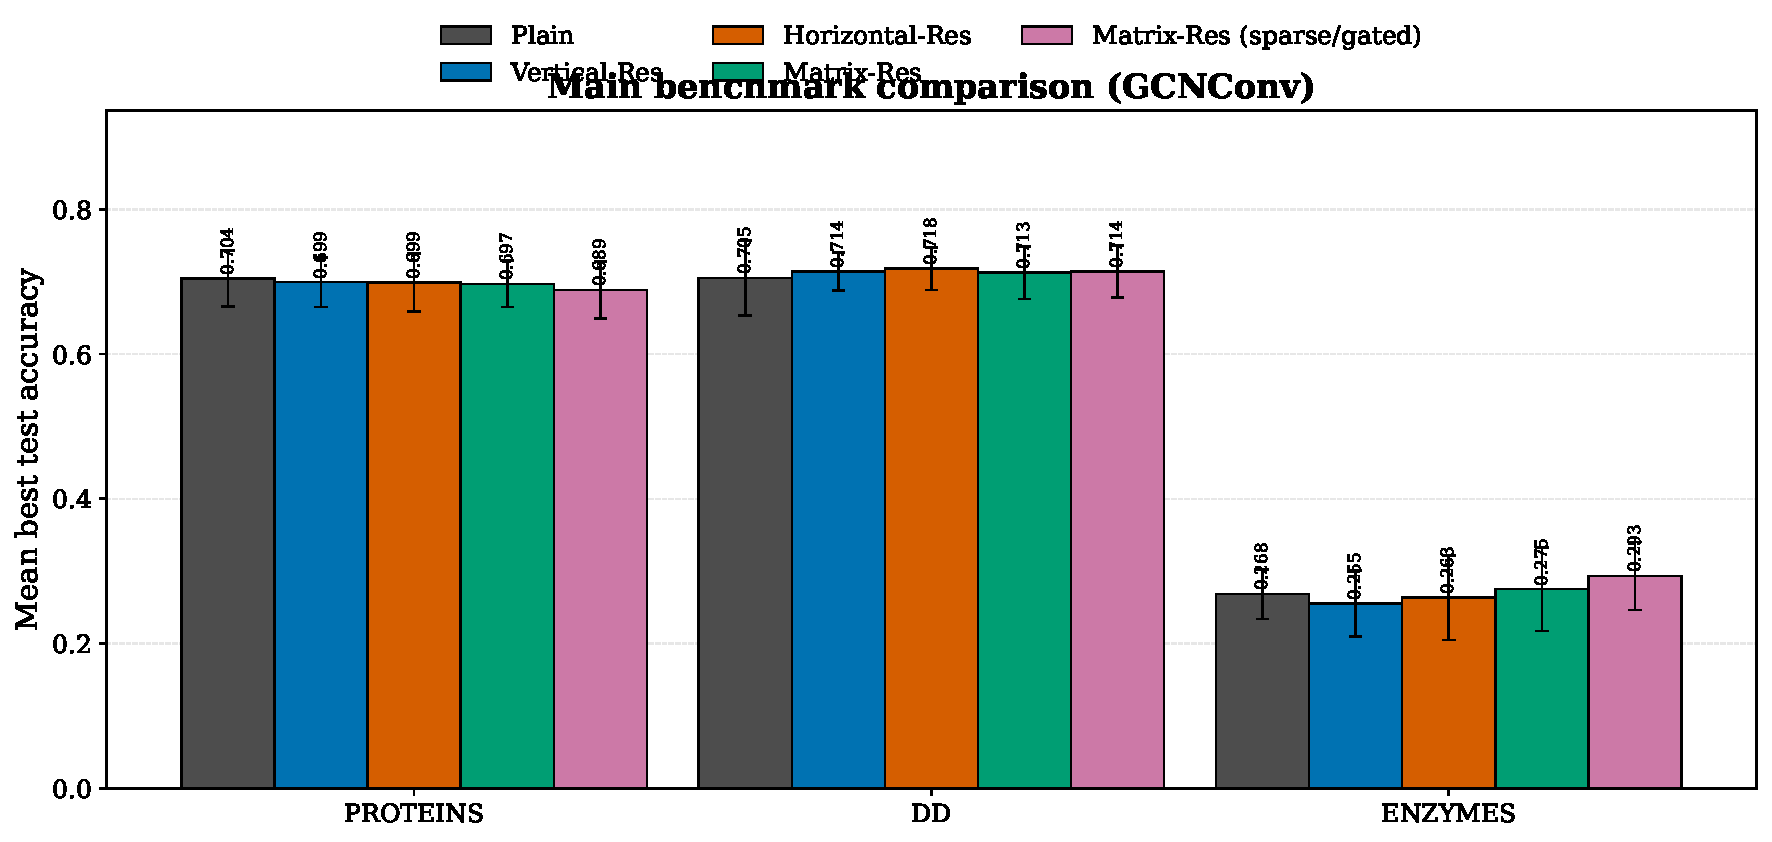
\includegraphics[width=0.92\linewidth]{figures/exp/fig_main_benchmark_gcnconv.pdf}
\caption{Main GCNConv benchmark at \(B=3\). Bars show five-fold mean best test accuracy with fold-level standard-deviation error bars.}
\label{fig:main_benchmark}
\end{figure}

Figure~\ref{fig:main_benchmark} makes the split regime visually explicit. The default GCNConv setting does not support a universal residual winner; instead, each dataset favors a different residual neighborhood.

\subsection{Operator robustness}

The full four-operator benchmark tests whether the GCNConv pattern is operator-specific. Table~\ref{tab:operator_wins} counts the winning topology across the 24 dataset--operator combinations. MatrixRes is the most frequent winner overall and wins under every operator family, but the remaining wins are distributed across all other models. This confirms that the residual-topology question is not reducible to one backbone choice.

\begin{table}[h]
\centering
\small
\caption{Winner counts across 24 dataset--operator combinations.}
\label{tab:operator_wins}
\begin{tabular}{l c c}
\toprule
Model & Wins & Mean rank \\
\midrule
Plain & 5 & 3.04 \\
VerticalRes & 2 & 3.38 \\
HorizontalRes & 3 & 3.54 \\
MatrixRes & \(\mathbf{9}\) & \(\mathbf{2.13}\) \\
MatrixResGated & 5 & 2.92 \\
\bottomrule
\end{tabular}
\end{table}

\begin{figure}[H]
\centering
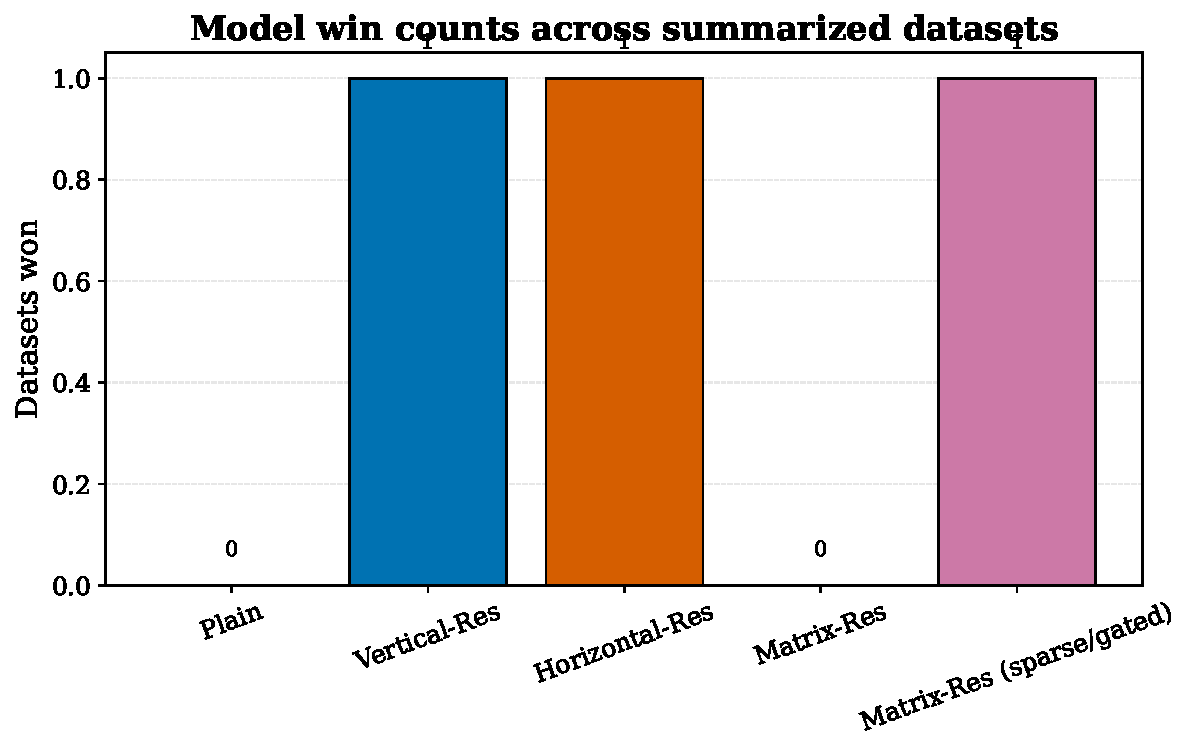
\includegraphics[width=0.82\linewidth]{figures/exp/fig_model_win_counts.pdf}
\caption{Model-level winner counts across the six datasets and four message-passing operators.}
\label{fig:model_win_counts}
\end{figure}

\subsection{Branch-count ablation}

Branch count has a non-monotonic effect. Table~\ref{tab:branch_best} reports the best branch count for each topology in the ablation. On PROTEINS, HorizontalRes peaks at \(B=4\), MatrixRes peaks at \(B=6\), and MatrixResGated peaks at \(B=3\). On DD, the preferred branch budget is smaller: HorizontalRes and MatrixRes peak at \(B=2\), while MatrixResGated is strongest at \(B=1\).

\begin{table}[h]
\centering
\small
\caption{Best branch-count setting for each topology in the ablation.}
\label{tab:branch_best}
\begin{tabular}{l l c c}
\toprule
Dataset & Model & Best \(B\) & Accuracy \\
\midrule
PROTEINS & HorizontalRes & 4 & \(0.7125\pm0.0286\) \\
PROTEINS & MatrixRes & 6 & \(0.7062\pm0.0210\) \\
PROTEINS & MatrixResGated & 3 & \(0.7098\pm0.0219\) \\
DD & HorizontalRes & 2 & \(0.7275\pm0.0304\) \\
DD & MatrixRes & 2 & \(0.7206\pm0.0411\) \\
DD & MatrixResGated & 1 & \(0.7283\pm0.0244\) \\
\bottomrule
\end{tabular}
\end{table}

\begin{figure}[H]
\centering
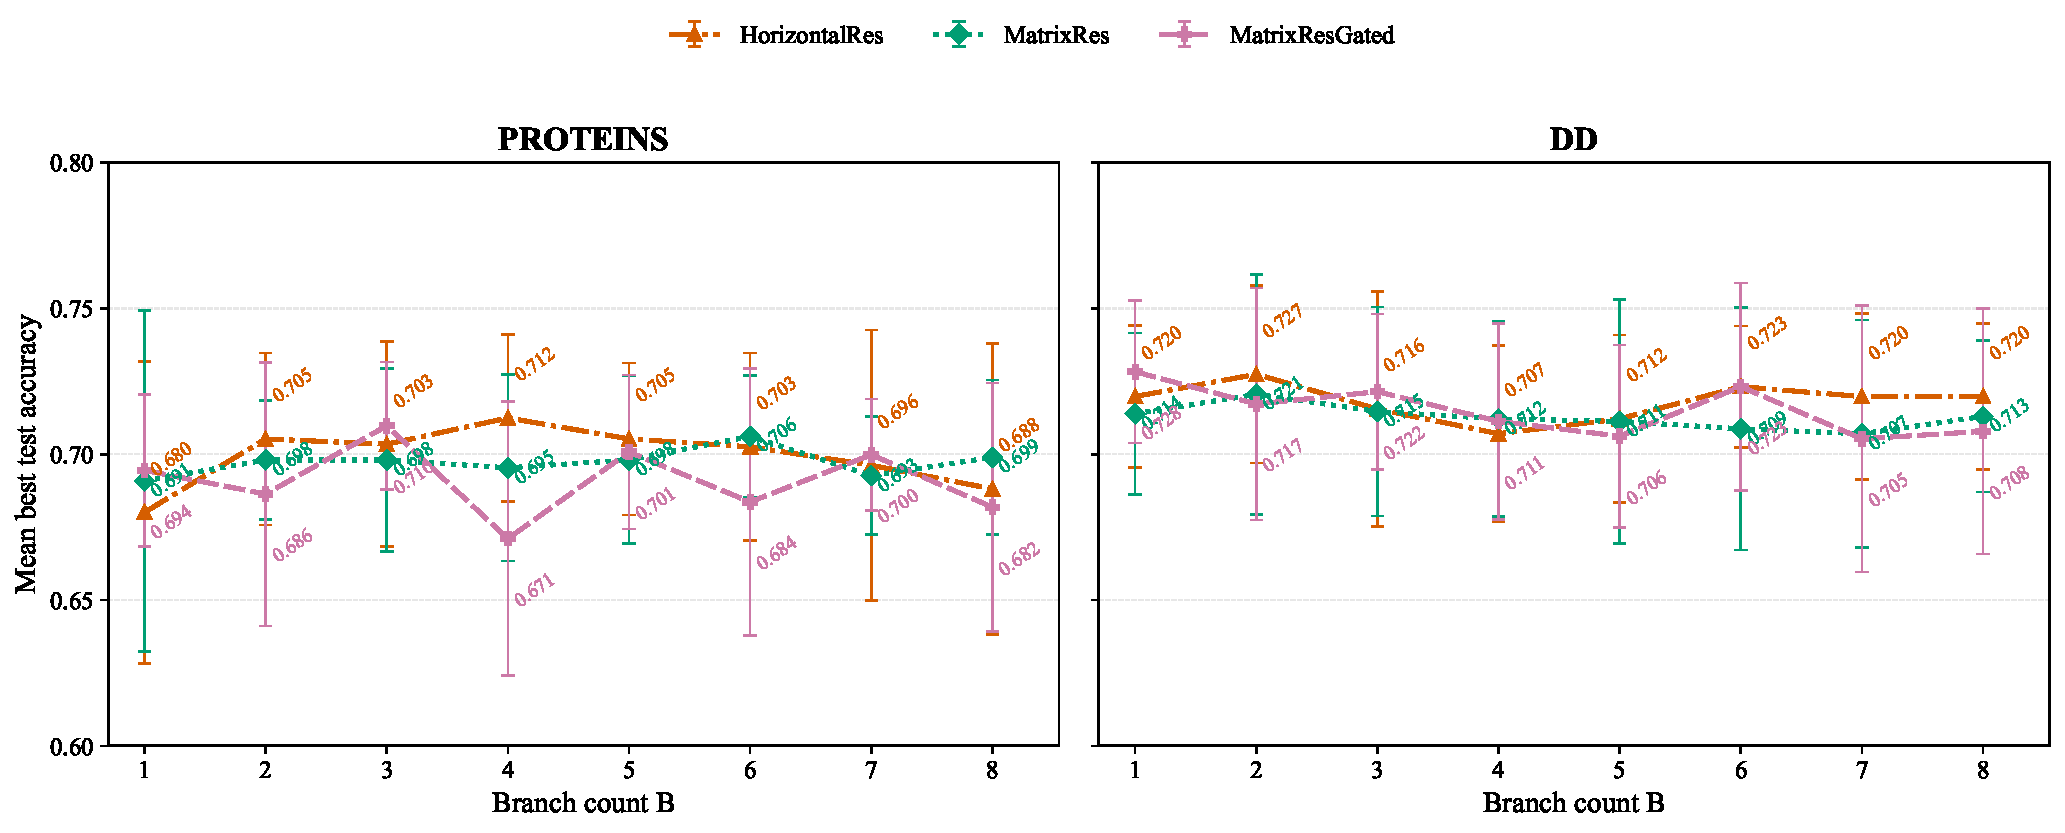
\includegraphics[width=0.92\linewidth]{figures/exp/fig_branch_count_ablation.pdf}
\caption{Branch-count ablation for HorizontalRes, MatrixRes, and MatrixResGated on PROTEINS and DD. Accuracy improves only within a useful operating region and then saturates or declines.}
\label{fig:branch_ablation}
\end{figure}

The ablation shows that branch count should not be read as a simple capacity knob. Increasing \(B\) changes the residual graph itself: it adds branches, residual paths, residual traffic, and optimization interactions. PROTEINS tolerates a moderate branch budget, while DD is more sensitive to redundant branch expansion.

\subsection{MatrixResGated sensitivity}

The fold-0 sensitivity scan shows that MatrixResGated is tunable, but its preferred region differs between datasets. On PROTEINS, the baseline MatrixResGated configuration reaches \(0.6726\), and mild sparsification with \(\lambda=0.02\) improves fold-0 accuracy to \(0.6951\). Stronger sparsification with \(\lambda=0.1\) reduces accuracy to \(0.6278\). On DD, the baseline fold-0 score is \(0.7300\), while \(lr=0.001\), \(dim=32\), and \(gate\_init=0.2\) each reach \(0.7511\).

\begin{table}[h]
\centering
\small
\caption{Strongest MatrixResGated fold-0 sensitivity settings.}
\label{tab:sensitivity}
\begin{tabular}{l l c l}
\toprule
Dataset & Setting & Accuracy & Interpretation \\
\midrule
PROTEINS & baseline & 0.6726 & default controlled matrix reuse \\
PROTEINS & \(\lambda=0.02\) & 0.6951 & mild sparsification improves fold 0 \\
PROTEINS & \(\lambda=0.1\) & 0.6278 & strong sparsification is harmful \\
DD & baseline & 0.7300 & default controlled matrix reuse \\
DD & \(lr=0.001\) & 0.7511 & conservative optimization helps \\
DD & \(dim=32\) & 0.7511 & smaller hidden dimension helps \\
DD & \(gate\_init=0.2\) & 0.7511 & lower initial gate helps \\
\bottomrule
\end{tabular}
\end{table}

\begin{figure}[H]
\centering
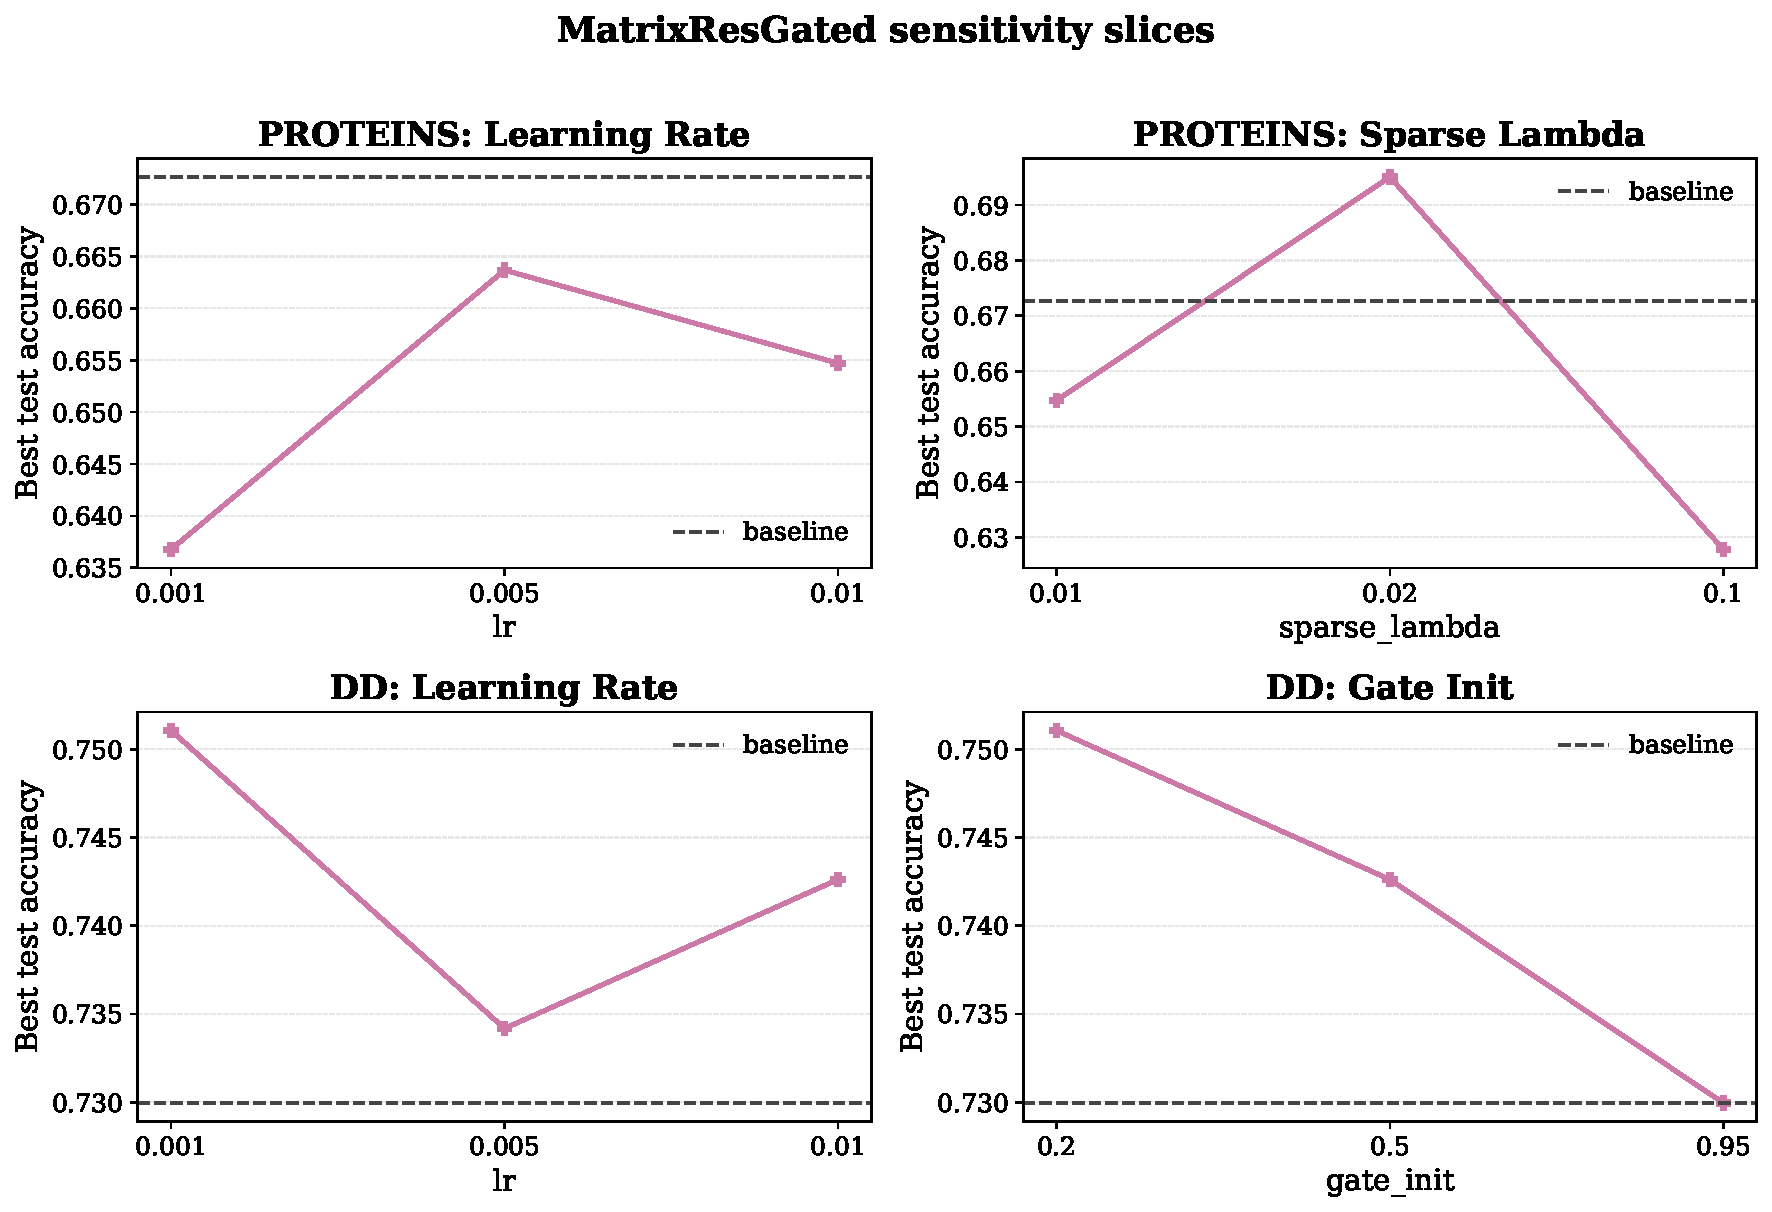
\includegraphics[width=0.92\linewidth]{figures/exp/fig_matrixresgated_sensitivity.pdf}
\caption{Fold-0 MatrixResGated sensitivity scan at \(B=3\). The scan identifies candidate operating regions but is not treated as final hyperparameter evidence.}
\label{fig:sensitivity}
\end{figure}

\subsection{Five-fold check of tuned MatrixResGated candidates}

To distinguish candidate discovery from evaluation, selected MatrixResGated settings were rerun across all five folds. Table~\ref{tab:tuned_candidates} reports these follow-up checks. On DD, the smaller hidden dimension is the strongest tuned candidate, reaching \(0.7215\pm0.0330\) while reducing parameters from 42,371 to 15,043. The lower learning rate is essentially tied with the default MatrixResGated benchmark, and the lower gate initialization is weaker. On PROTEINS, \(\lambda=0.02\) reaches \(0.6909\pm0.0447\), below the default MatrixResGated result, showing that the fold-0 sparsity gain is not stable across all folds in the current run.

\begin{table}[h]
\centering
\small
\caption{Five-fold checks of selected MatrixResGated candidates.}
\label{tab:tuned_candidates}
\begin{tabular}{l l c c c}
\toprule
Candidate & Dataset & Accuracy & Mean loss & Parameters \\
\midrule
\texttt{PROTEINS\_sparse\_lambda\_0.02} & PROTEINS & \(0.6909\pm0.0447\) & 0.6104 & 38,339 \\
\texttt{DD\_lr\_0.001} & DD & \(0.7181\pm0.0336\) & 0.5737 & 42,371 \\
\texttt{DD\_dim\_32} & DD & \(\mathbf{0.7215\pm0.0330}\) & 0.5717 & 15,043 \\
\texttt{DD\_gate\_init\_0.2} & DD & \(0.7131\pm0.0213\) & 0.5820 & 42,371 \\
\bottomrule
\end{tabular}
\end{table}

\subsection{Mechanism analysis}

The mechanism summaries support a common explanation for the rise-then-fall trend. Increasing branch count initially creates useful diversity: branches become less identical and can cover complementary feature subspaces. Past the useful regime, diversity alone is not sufficient. Residual traffic grows quickly, branch similarity may remain high, and gradient norms can weaken.

For HorizontalRes on PROTEINS, moving from \(B=1\) to \(B=4\) increases branch diversity from 0.0000 to 1.1450, while branch cosine decreases from 1.0000 to 0.8417. This corresponds to the accuracy improvement. Beyond \(B=4\), diversity continues increasing, reaching 1.5441 at \(B=8\), but accuracy declines to 0.6881. MatrixRes shows a similar trend at a larger branch budget, peaking at \(B=6\). DD is more conservative: branch expansion beyond \(B=2\) often adds residual complexity without enough functional separation.

\begin{figure}[H]
\centering
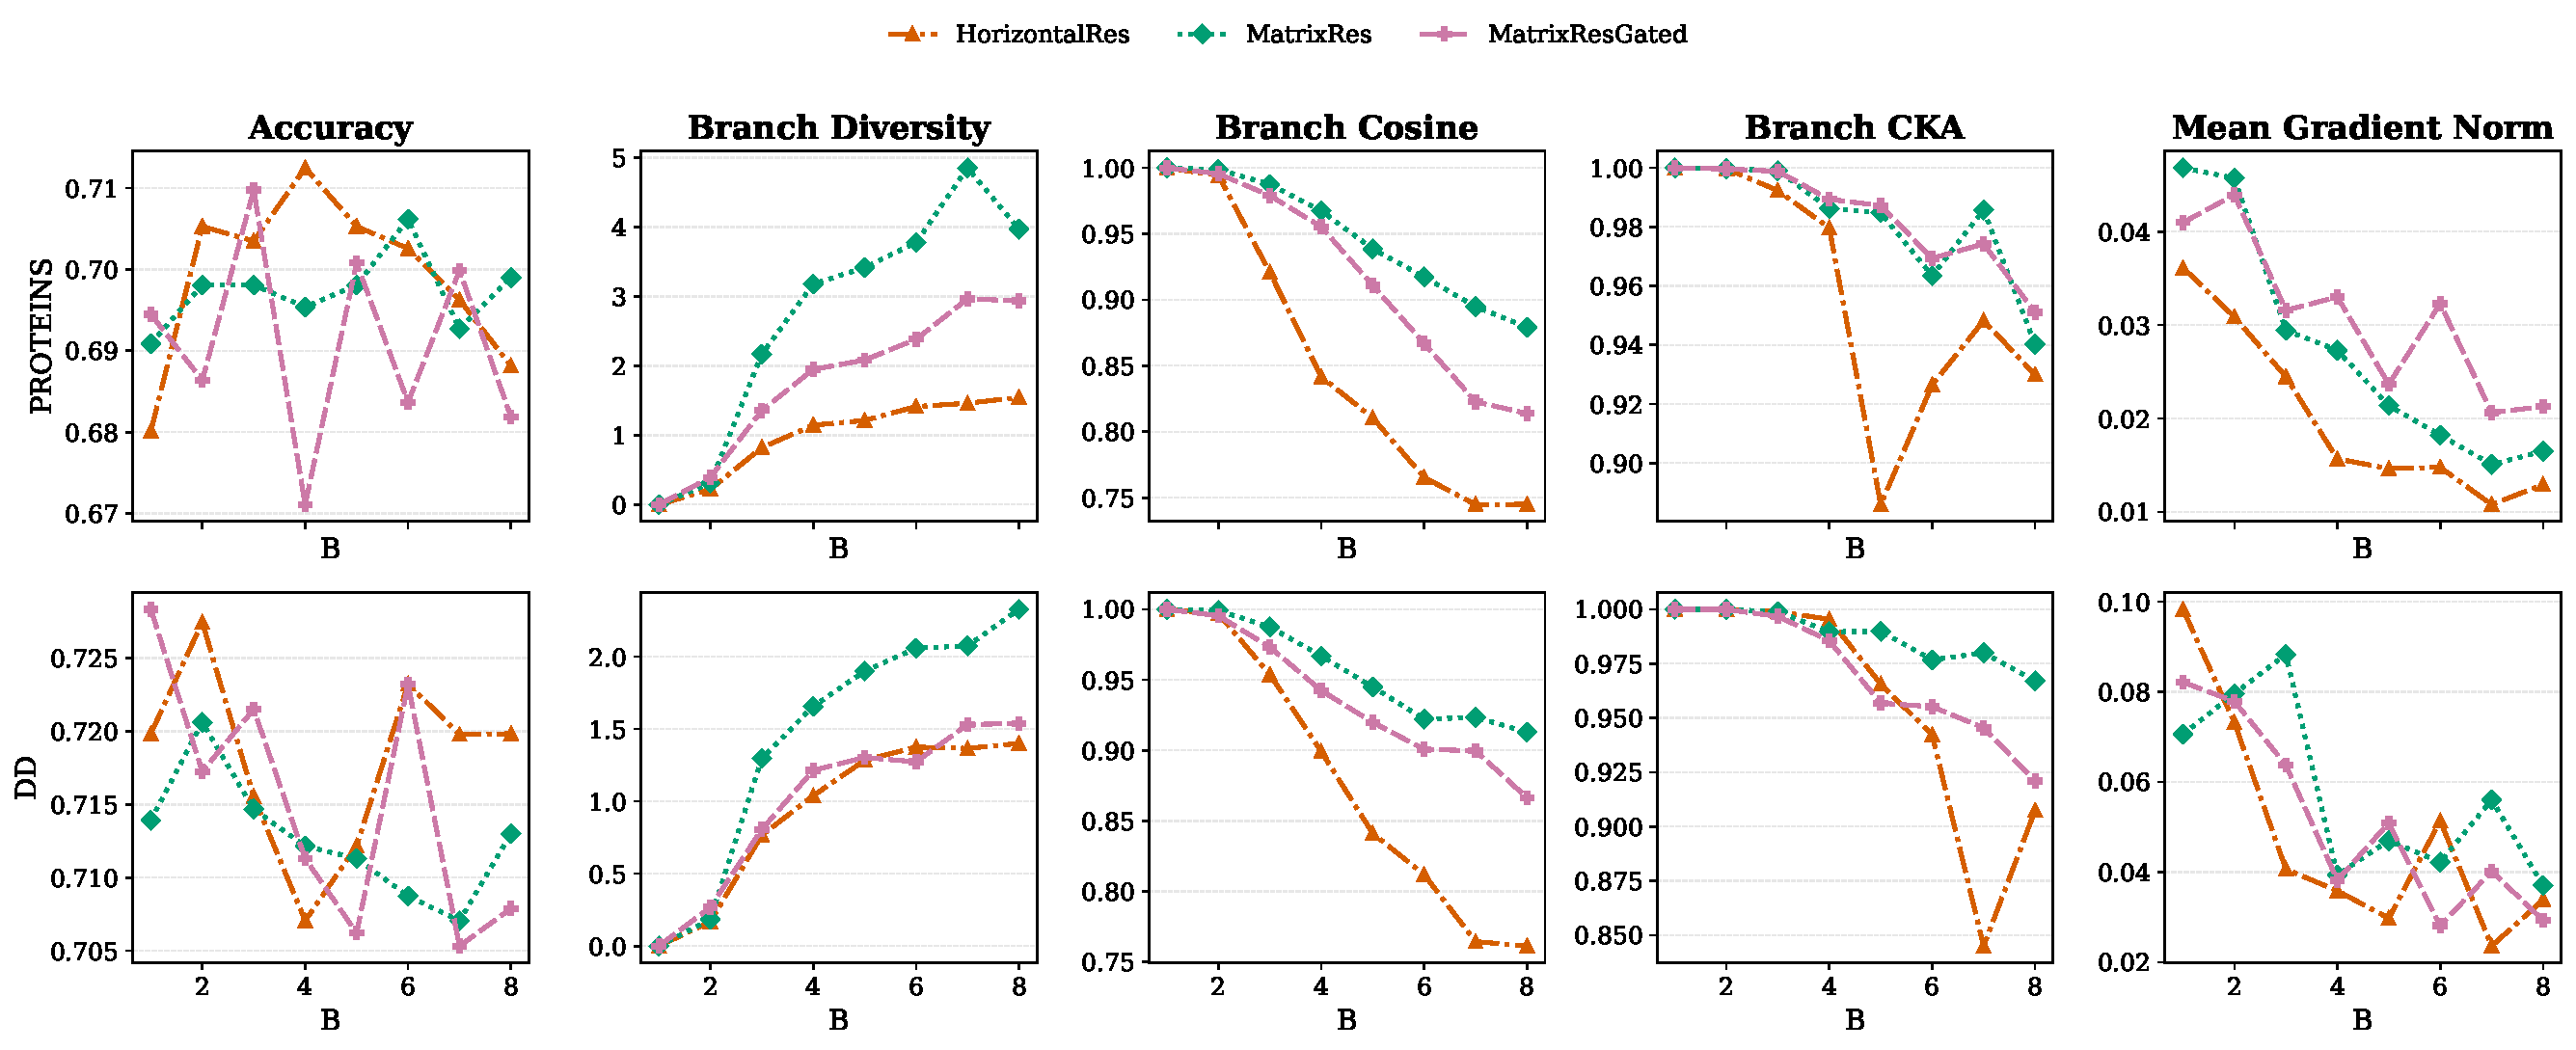
\includegraphics[width=0.92\linewidth]{figures/exp/fig_mechanism_branch_dynamics.pdf}
\caption{Mechanism summary linking branch-count accuracy to branch diversity, branch cosine similarity, and mean gradient norm.}
\label{fig:mechanism}
\end{figure}

\section{Discussion}

This section answers the three research questions in light of the benchmark, ablation, tuned-candidate, and mechanism evidence.

\subsection{RQ1: Which residual topology is strongest?}

The main benchmark argues against a universal residual topology. At \(B=3\), HorizontalRes is strongest on PROTEINS, VerticalRes is strongest on DD, and MatrixResGated is strongest on ENZYMES. These outcomes indicate that the useful residual neighborhood depends on dataset-specific tolerance for branch specialization, residual traffic, and optimization complexity.

\textbf{Answer:} Residual topology is dataset-dependent. A graph-classification benchmark should compare vertical, horizontal, and matrix-style reuse rather than assuming that one residual direction is universally best.

\subsection{RQ2: How does branch count change residual behavior?}

The branch-count ablation shows that \(B\) is not only a capacity parameter. Increasing \(B\) adds branches, residual paths, and optimization interactions. On PROTEINS, moderate expansion is useful: HorizontalRes peaks at \(B=4\), MatrixRes at \(B=6\), and MatrixResGated at \(B=3\). On DD, smaller budgets are preferable, with peaks at \(B=1\) or \(B=2\). The mechanism summaries explain this split. Branch diversity may increase with \(B\), but if branch cosine remains high or gradients weaken, the extra branches do not translate into better classification.

\textbf{Answer:} Branch count helps when it creates useful functional diversity, and hurts when residual complexity grows faster than branch separation or optimization quality.

\subsection{RQ3: When does controlled matrix reuse help?}

MatrixResGated defines a tunable family rather than a plug-and-play winner. The fold-0 sensitivity scan suggests that PROTEINS can benefit from mild sparsification, while DD benefits from conservative optimization, smaller hidden dimension, and lower initial gate. The five-fold candidate reruns refine this interpretation. On DD, the smaller hidden dimension remains beneficial and parameter-efficient. On PROTEINS, the mild-sparsity candidate does not preserve its fold-0 advantage across all folds.

\textbf{Answer:} Controlled matrix reuse is useful, but candidate settings must be validated across folds. The current evidence supports a smaller controlled matrix model on DD and leaves PROTEINS sparsification as a promising but not yet stable direction.

\subsection{Limitations}

Several limitations bound the generality of these findings. First, the main benchmark uses GCNConv only. This makes the comparison controlled but leaves open whether the same residual-topology trends hold for GINConv, GraphSAGE, or attention-based operators. Second, the sensitivity scan is fold-0 only; although selected candidates were rerun across five folds, that follow-up is limited to MatrixResGated on PROTEINS and DD. Third, ENZYMES has low absolute accuracy and high variability, so its result should be interpreted cautiously. Finally, the mechanism analysis is correlational. Branch diversity, cosine similarity, and gradient norms support a coherent explanation, but they do not prove causality.

\subsection{Future directions}

Future work should extend the comparison to additional message-passing operators, larger graph-classification datasets, and adaptive residual-neighborhood selection. A natural next step is to replace manually chosen vertical, horizontal, or matrix stencils with a learned local residual policy. The tuned-candidate validation should also be broadened beyond the current MatrixResGated checks to determine whether dataset-specific residual control can be selected reliably.

\section{Conclusions}
\label{sec:conclusion}

This paper studies residual connectivity for graph classification as a structured branch-by-layer design problem. Across six datasets and four message-passing operators, residual topology matters, but its value depends on the dataset, operator, and branch budget. MatrixRes is the most frequent winner and has the best mean rank in the full benchmark, but the per-dataset GCNConv winners remain mixed: Plain is strongest on PROTEINS, HorizontalRes on DD, MatrixResGated on ENZYMES, and MatrixRes on MUTAG, AIDS, and Mutagenicity. The ENZYMES comparison has low absolute accuracy and should be interpreted cautiously. The branch-count ablations further show that adding branches is useful only within a limited operating region.

The mechanism analysis provides a plausible explanation for why branch expansion is not automatically beneficial. Additional branches can increase representational diversity, but they also increase residual traffic and may preserve redundant branch similarity or weaken optimization. Matrix-style reuse is best viewed as a controlled residual family whose effectiveness depends on the branch budget and residual filtering strategy.

The practical implication is that residual topology, branch count, operator choice, and residual control should be evaluated jointly. Before treating a sensitivity result as a performance claim, candidate settings should be rerun across folds. In the current experiments, this validation supports a smaller and more parameter-efficient MatrixResGated model on DD, while the PROTEINS sparsity candidate remains less stable.

\input{sections/06_acknowledgments.tex}
\appendix

\section{Appendix}
\label{sec:appendix}

\subsection{Result sources}

The manuscript uses the following summary files as the source of truth. The main benchmark summary contains 120 model-level rows: six datasets, four operators, five model families, and five-fold aggregation for each combination.
\begin{itemize}
    \item \texttt{records/LATEST/summaries/benchmark\_summary.csv}
    \item \texttt{records/LATEST/summaries/branch\_ablation\_summary.csv}
    \item \texttt{records/LATEST/summaries/parameter\_sensitivity\_summary.csv}
    \item \texttt{records/LATEST/summaries/tuned\_candidate\_summary.csv}
    \item \texttt{records/LATEST/summaries/mechanism\_compact\_summary.csv}
    \item \texttt{records/SYN\_MULTI\_FULL/summaries/benchmark\_summary.csv}
\end{itemize}

\subsection{Supplementary diagnostics}

Additional fold-level rows, CKA summaries, residual traffic summaries, and full sensitivity tables are retained in the repository records directory for supplementary conversion.

\subsection{Evidence map}

Table~\ref{tab:evidence_map} summarizes where each main empirical claim is supported in the manuscript. This compact table is included to keep the main text readable while still making the result-to-claim link explicit.

\begin{table}[h]
\centering
\small
\caption{Compact map from empirical claims to manuscript evidence.}
\label{tab:evidence_map}
\begin{tabular}{p{0.42\linewidth} p{0.44\linewidth}}
\toprule
Claim & Primary evidence \\
\midrule
MatrixRes is the most frequent winner in the full benchmark but not a universal winner. & Table~\ref{tab:operator_wins}, Table~\ref{tab:winners_by_operator}, and Figure~\ref{fig:model_win_counts}. \\
GCNConv results remain dataset-dependent under a fixed operator. & Table~\ref{tab:main_benchmark} and Figure~\ref{fig:main_benchmark}. \\
Branch count produces a rise-then-fall pattern rather than monotonic improvement. & Table~\ref{tab:branch_best} and Figure~\ref{fig:branch_ablation}. \\
Useful branch expansion is associated with separation without excessive residual traffic. & Table~\ref{tab:mechanism_snapshot} and Figure~\ref{fig:mechanism}. \\
Fold-0 sensitivity should not be treated as final evidence. & Table~\ref{tab:sensitivity}, Figure~\ref{fig:sensitivity}, and Table~\ref{tab:tuned_candidates}. \\
Matrix-style reuse becomes more favorable in higher-class synthetic structural discrimination. & Table~\ref{tab:synthetic_class_scaling}, Figure~\ref{fig:synthetic_multiclass_scaling}, Table~\ref{tab:synthetic_high_class}, and Table~\ref{tab:synthetic_distribution_high_class}. \\
\bottomrule
\end{tabular}
\end{table}

\subsection{Synthetic distribution-level summary}

Table~\ref{tab:synthetic_distribution_high_class} reports the higher-class synthetic results by graph family. The table is placed in the appendix because the main text focuses on the class-count scaling trend. It shows that MatrixRes is strongest on BA, ER, and random-regular graphs, while SBM and WS remain less favorable to matrix-style reuse.

\begin{table}[h]
\centering
\scriptsize
\caption{Synthetic high-class accuracy by graph family, averaged over \(C=4,\ldots,8\) and four operators.}
\label{tab:synthetic_distribution_high_class}
\begin{tabular}{l c c c c c}
\toprule
Family & Plain & VerticalRes & HorizontalRes & MatrixRes & MatrixResGated \\
\midrule
BA & 0.7874 & 0.8177 & 0.7855 & \(\mathbf{0.8271}\) & 0.8257 \\
ER & 0.8777 & 0.8756 & 0.8728 & \(\mathbf{0.8807}\) & 0.8796 \\
Regular & 0.7505 & 0.7923 & 0.7739 & \(\mathbf{0.8077}\) & 0.8057 \\
SBM & 0.6268 & \(\mathbf{0.6286}\) & 0.6218 & 0.6264 & 0.6176 \\
WS & \(\mathbf{0.3709}\) & 0.3511 & 0.3693 & 0.3202 & 0.3430 \\
\bottomrule
\end{tabular}
\end{table}


\bibliographystyle{plainnat}
\bibliography{references}

\end{document}
